\subsection{n-gram 構成方式と stop words 設計の定量比較}

課題 6 の実装では、(1) 正規表現 {\tt [a-z]+} によるトークン化、
(2) 自作の stop words 集合による語の除去、(3) 除去後の単語列からの
2-gram 構成、という 3 段階の設計を採用した。先に定性的に指摘した
「e g」の出現原因と 2-gram 構成方式の影響を定量的に裏付け、さらに
n-gram の次数 $n$ と stop words 集合の規模が結果に与える影響を
明らかにするため、追加実験(実験ソースは付録の
{\tt exp05\_ngram\_design.py}、実行出力は付録の {\tt exp05.txt})を
行った。対象は課題と同一の text\_english.txt であり、トークン化の
結果は総トークン数 984、異なり語数 445 である。提出プログラムの
{\tt STOP\_WORDS} は 86 語からなり、以下では「採用集合」と呼ぶ。
トークン化と n-gram 構成の実装は提出プログラムと同一仕様とし、
順位付けは頻度降順・同数の場合は辞書順として決定的に定めた。

\subsubsection{2-gram 構成方式の比較}

stop words 除去と 2-gram 構成の順序が異なる次の 2 方式を比較した。

\begin{enumerate}
\item 方式 A: stop words を除去した後の単語列から 2-gram を構成する
      (提出プログラムの採用手法)。
\item 方式 B: 原文の単語列から 2-gram を構成した後、2 語のどちらかが
      stop word である組を除去する。
\end{enumerate}

方式 A は stop words を挟んで離れていた 2 語を新たな隣接ペアとして
数えるのに対し、方式 B は原文でトークンが隣接していた組だけを数える。
両方式の上位 10 を表 \ref{tab:b5-methods} と図 \ref{fig:b5-methods} に
示す。

\begin{table}[htbp]
\centering
\caption{2-gram 構成方式別の上位 10(頻度降順、同数は辞書順)}
\label{tab:b5-methods}
\begin{tabular}{rlrlr}
\hline
順位 & 方式 A(採用) & 頻度 & 方式 B & 頻度 \\
\hline
1 & natural language & 15 & natural language & 15 \\
2 & e g & 9 & e g & 9 \\
3 & language processing & 9 & language processing & 9 \\
4 & machine translation & 5 & machine translation & 5 \\
5 & language understanding & 3 & language understanding & 3 \\
6 & machine learning & 3 & machine learning & 3 \\
7 & annotated data & 2 & annotated data & 2 \\
8 & artificial intelligence & 2 & artificial intelligence & 2 \\
9 & g development & 2 & head hurts & 2 \\
10 & generation natural & 2 & language data & 2 \\
\hline
\end{tabular}
\end{table}

\begin{figure}[htbp]
\centering
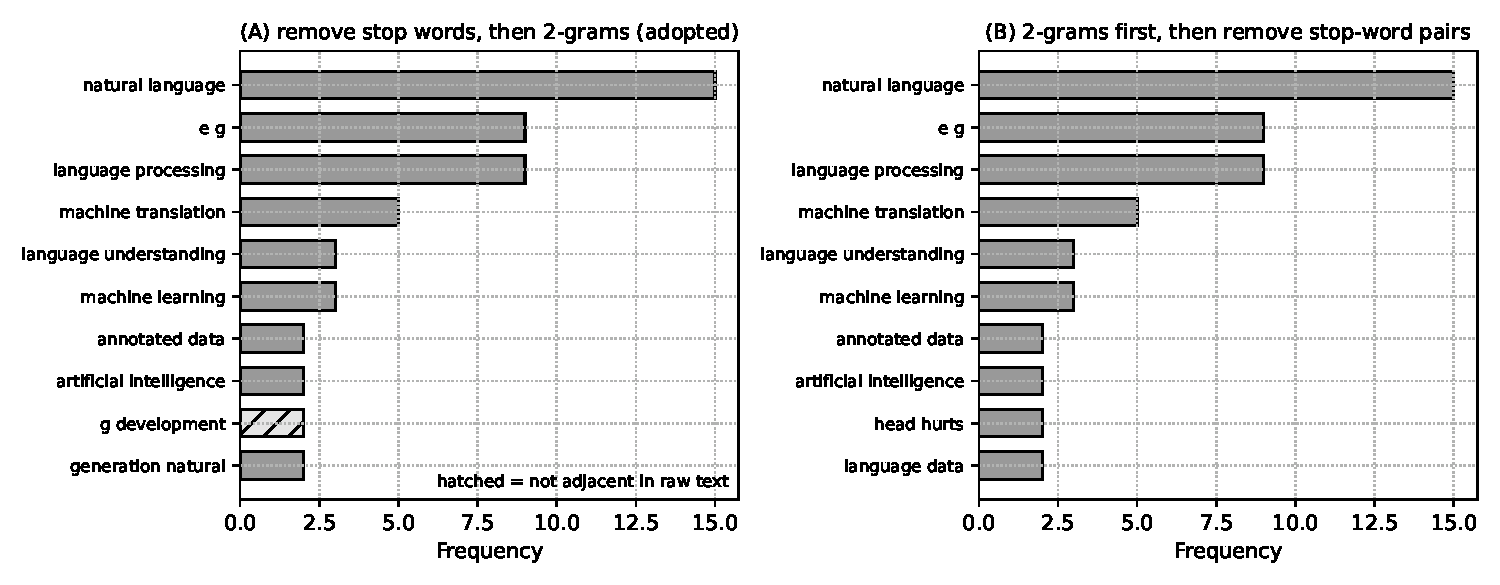
\includegraphics[width=0.98\linewidth]{../experiments/figures/exp05_methods.pdf}
\caption{2-gram 構成方式別の上位 10。左が方式 A(採用)、右が方式 B で
あり、ハッチ付きの棒は原文に隣接ペアとして存在しない組を表す。}
\label{fig:b5-methods}
\end{figure}

全体の集計では、方式 A の 2-gram は総数 613・異なり数 560、方式 B は
総数 347・異なり数 300 であり、方式 B の総数は方式 A の 56.6 \% に
とどまる。両者の総数の差 266 個が、stop words を挟んで新たに生成された
隣接ペアの実数である。このうち 262 個(方式 A の総数の 42.7 \%)は、
原文に隣接ペアとして一度も現れない組(異なり数で 260/560、46.4 \%)に
属する。すなわち方式 A が数えるペアの 4 割強は、原文には連接として
存在しない「stop words 越しの共起」である。

一方、表 \ref{tab:b5-methods} のとおり上位 10 に限れば両方式の
1〜8 位は頻度まで完全に一致し、相違は 9 位以下の頻度 2 の組にのみ
現れた。方式 A の 9 位「g development」(頻度 2)は原文に隣接ペアと
して存在せず、方式 B では頻度 0 である。これは原文の
「e.g., the development」(2 箇所)がトークン化で e / g / the /
development に分割され、the の除去によって g と development が
隣接した人工的な組である。また方式 A の 10 位「generation natural」
(頻度 2)は、方式 B では頻度 1・順位 98 に後退する。方式 A における
頻度 2 の内訳は、1 回が「generation of natural」の of 除去による
非隣接ペア、もう 1 回が文境界をまたぐトークンの隣接
(前文末尾の generation と次文先頭の Natural)である。後者は、
句読点を捨てるトークン化では文境界の情報も失われ、隣接だけを数える
方式 B でも文をまたぐ組が集計されることを示している。

以上から、両方式の違いは頻度 2 以下の低頻度域に集中し、本テキストの
規模では主要な内容語ペア(上位 8)の抽出結果は方式の選択に対して
頑健であることが定量的に確認できた。ただし方式 A の全ペアの
42.7 \% は原文に実在しない連接であるから、抽出した 2-gram を
「原文に現れる表現」として提示する用途では方式 B を、stop words を
越えた共起関係を広く拾う用途では方式 A を使うべきであり、
両方式は目的に応じた使い分けを要する設計選択である。

\subsubsection{n-gram の次数と情報量}

次数 $n$ を 1, 2, 3 と変え、stop words 除去(採用集合で除去後に構成)の
あり/なしの計 6 通りで上位 10 と統計量を集計した。上位 10 を
図 \ref{fig:b5-ngrams} に、統計量を表 \ref{tab:b5-ngram-stats} に示す。
表中のハパックス率は頻度 1 の n-gram が異なり数に占める割合、
上位 10 被覆率は上位 10 の頻度合計が n-gram 総数に占める割合である。

\begin{table}[htbp]
\centering
\caption{n-gram の次数別の統計量(text\_english.txt、除去は採用集合 86 語)}
\label{tab:b5-ngram-stats}
\begin{tabular}{clrrrr}
\hline
stop words & $n$ & 総数 & 異なり数 & ハパックス率 [\%] & 上位 10 被覆率 [\%] \\
\hline
除去なし & 1 & 984 & 445 & 71.7 & 27.1 \\
除去なし & 2 & 983 & 858 & 92.9 & 7.5 \\
除去なし & 3 & 982 & 958 & 98.5 & 3.1 \\
除去あり & 1 & 614 & 389 & 76.9 & 16.9 \\
除去あり & 2 & 613 & 560 & 96.2 & 8.5 \\
除去あり & 3 & 612 & 599 & 98.8 & 3.8 \\
\hline
\end{tabular}
\end{table}

\begin{figure}[htbp]
\centering
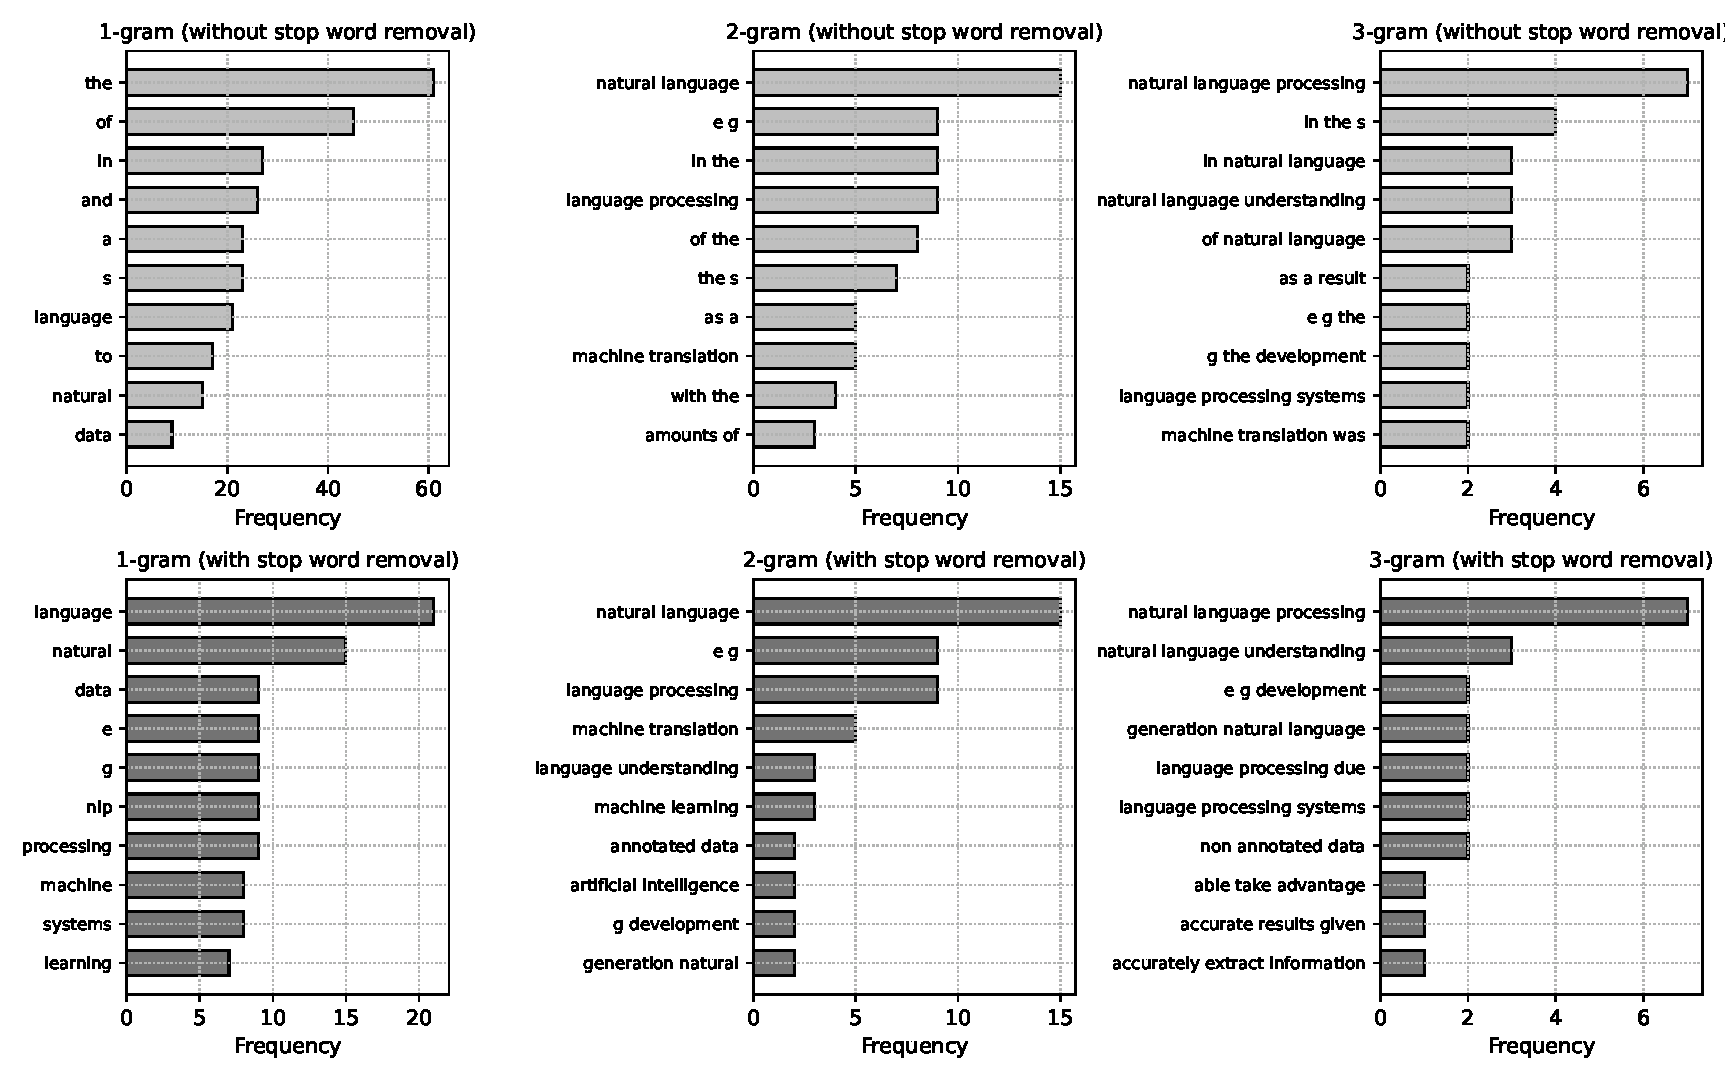
\includegraphics[width=\linewidth]{../experiments/figures/exp05_ngram_bars.pdf}
\caption{n-gram の次数別の上位 10。上段が stop words 除去なし、
下段が除去あり(採用集合 86 語)、左から $n = 1, 2, 3$ である。}
\label{fig:b5-ngrams}
\end{figure}

$n = 1$(除去なし)の上位 10 は the(61 回)、of(45 回)、in(27 回)
など機能語とトークン断片 {\tt s}(23 回、1950s などの数字除去で生じる)
が 7 枠を占め、内容語は language(21 回)、natural(15 回)、
data(9 回)の 3 語にとどまる。除去ありの $n = 1$ では主題語が並ぶが、
language と processing がひとまとまりの概念であるという語順の情報は
得られない。$n = 2$ になると語順の情報が加わり、除去ありの上位は
natural language、language processing、machine translation、
machine learning、artificial intelligence と、テキストの主題を表す
複合語・術語で占められる。$n = 3$ ではさらに特定的な表現
(natural language processing 7 回、natural language understanding
3 回)が得られる。

一方、表 \ref{tab:b5-ngram-stats} のとおり、$n$ の増加とともに
異なり数は 445 → 858 → 958(除去なし)と増え、ハパックス率は
71.7 \% → 92.9 \% → 98.5 \% に達する。上位 10 被覆率は
27.1 \% → 7.5 \% → 3.1 \% と急落し、除去ありの $n = 3$ では
上位 10 の 8 位以下が頻度 1 の組で占められて、頻度に基づく順位付けが
実質的に機能しなくなる。すなわち $n$ の増加は 1 つの n-gram が担う
情報量(表現の特定性)を高める一方で、各 n-gram の出現頻度を急速に
希薄化させる。総トークン数 984 の本テキストでは、頻度統計として
意味のある上位比較が成立するのは $n = 2$ までであり、課題の 2-gram
という設定はこのコーパス規模に対して妥当な選択であるといえる。

\subsubsection{Zipf 則の検証}

自然言語の語頻度分布では、頻度 $f$ と頻度順位 $r$ の間に

\begin{equation}\label{eq:b5-zipf}
f(r) = C r^{-s}
\end{equation}

という冪則(Zipf 則)が成り立ち、指数 $s$ は 1 に近い値をとることが
知られている \cite{b5-stanisz}。ここで $C$ は定数である。式
\ref{eq:b5-zipf} の両辺の常用対数をとると

\begin{equation}\label{eq:b5-zipf-log}
\log_{10} f = \log_{10} C - s \log_{10} r
\end{equation}

となり、log-log プロット上の回帰直線の傾きとして $-s$ を推定できる。
stop words を除去しない 1-gram(445 種)と 2-gram(858 種)の
頻度-順位分布を図 \ref{fig:b5-zipf} に、式 \ref{eq:b5-zipf-log} に
基づく最小二乗フィットの結果を表 \ref{tab:b5-zipf} に示す。フィットは
全点を用いる場合と、頻度 1 の階段状の裾を除いた頻度 2 以上の点のみを
用いる場合の 2 通りで行った。

\begin{table}[htbp]
\centering
\caption{頻度-順位分布の log-log 最小二乗フィットの結果}
\label{tab:b5-zipf}
\begin{tabular}{llrrr}
\hline
系列 & フィット範囲 & 点数 & 傾き $-s$ & 決定係数 $R^2$ \\
\hline
1-gram & 全点 & 445 & $-0.673$ & 0.897 \\
1-gram & 頻度 2 以上 & 126 & $-0.787$ & 0.971 \\
2-gram & 全点 & 858 & $-0.213$ & 0.569 \\
2-gram & 頻度 2 以上 & 61 & $-0.504$ & 0.884 \\
\hline
\end{tabular}
\end{table}

\begin{figure}[htbp]
\centering
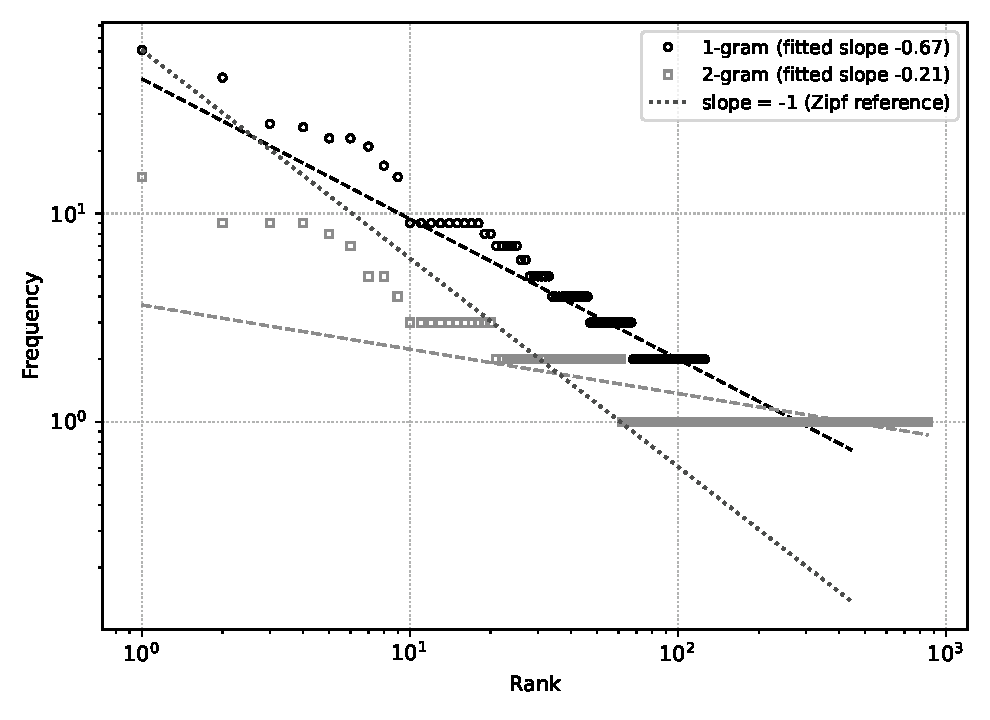
\includegraphics[width=0.72\linewidth]{../experiments/figures/exp05_zipf.pdf}
\caption{1-gram と 2-gram の頻度-順位分布(log-log)。破線は全点に
対する最小二乗フィット、点線は傾き $-1$(Zipf 則の理論値)の基準線で
ある。}
\label{fig:b5-zipf}
\end{figure}

推定された傾きの大きさはいずれも理論値 1 より小さい。1-gram では
全点フィットで $s = 0.673$、頻度 2 以上に限ると $s = 0.787$
($R^2 = 0.971$)となり、頭部の直線性は高いものの依然として 1 には
届かない。この浅さの主因はコーパス規模である。984 トークンに対して
異なり語が 445 あり、その 71.7 \% が頻度 1 であるため、図
\ref{fig:b5-zipf} の裾は頻度 1 の水平な階段になり、全点フィットの
傾きを押し上げる。2-gram ではこの効果がさらに顕著で、858 種の
92.9 \% がハパックスであり、冪則的な頭部はおよそ 20 位までしか
形成されない(全点フィットは $s = 0.213$、$R^2 = 0.569$ と直線近似
自体が成立しない)。単語頻度の Zipf 則は大規模コーパスで確認されて
きた統計則であり、句読点をトークンとして扱うか否かなどトークン化の
設計がスケーリングの成否に影響することも報告されている
\cite{b5-stanisz}。したがって本結果の浅い傾きは Zipf 則そのものの
破れではなく、約 1000 トークンという規模による分布の打ち切り
(有限サイズ効果)に、句読点・数字を捨てる本実装のトークン化の影響が
重なったものと解釈できる。課題 6 の観点では、上位 10 の頻度が
15, 9, 9, 5, $\ldots$ と急減すること自体が Zipf 型の偏りの現れであり、
少数の高頻度 n-gram だけでテキストの主題を要約できるという課題 6 の
アプローチの統計的根拠になっている。

\subsubsection{stop words 集合の設計に対する感度}

stop words 集合を、(i) 空集合、(ii) 冠詞・接続詞・be 動詞・頻出前置詞・
頻出代名詞のみからなる基本 30 語、(iii) 採用集合 86 語、(iv) 採用集合に
1 文字語 26 語(a〜z)を加えた 108 語、の 4 通りに変え、方式 A による
2-gram の上位 10 を比較した。結果を表 \ref{tab:b5-stopwords} と
図 \ref{fig:b5-stopwords} に示す。

\begin{table}[htbp]
\centering
\caption{stop words 集合別の 2-gram 統計と「e g」の順位}
\label{tab:b5-stopwords}
\begin{tabular}{lrrrrc}
\hline
集合 & 語数 & 除去後トークン数 & 異なり 2-gram 数 & 「e g」頻度 & 「e g」順位 \\
\hline
(i) なし & 0 & 984 & 858 & 9 & 2 \\
(ii) 基本 30 語 & 30 & 694 & 628 & 9 & 2 \\
(iii) 採用集合 & 86 & 614 & 560 & 9 & 2 \\
(iv) 採用 $+$ 1 文字語 & 108 & 596 & 551 & 0 & --- \\
\hline
\end{tabular}
\end{table}

\begin{figure}[htbp]
\centering
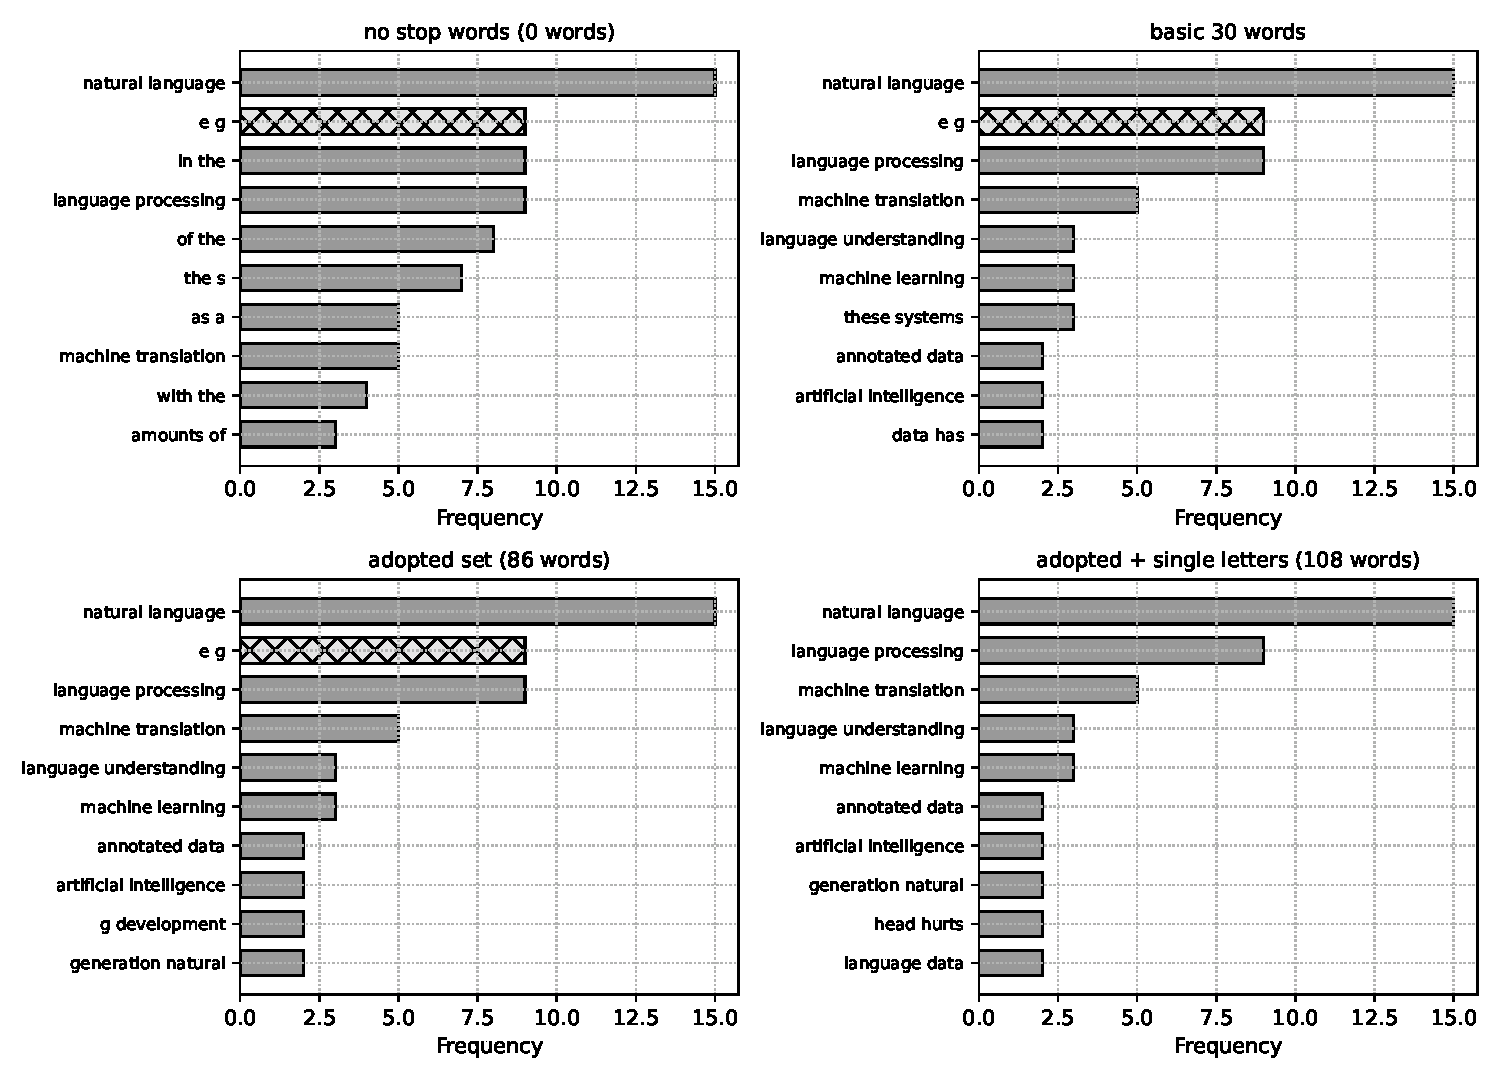
\includegraphics[width=0.95\linewidth]{../experiments/figures/exp05_stopwords.pdf}
\caption{stop words 集合別の 2-gram 上位 10(方式 A)。ハッチ付きの
棒は「e g」であり、1 文字語を追加した右下の集合でのみ消滅する。}
\label{fig:b5-stopwords}
\end{figure}

第一に、機能語ペアの排除効果は集合の最初の 30 語でほぼ決まる。
集合 (i) の上位 10 には in the(9 回)、of the(8 回)、the s(7 回)
など、採用集合の基準で stop word を含む組が 6 組入るが、集合 (ii) では
この 6 組がすべて上位 10 から消え、採用集合との違いは these systems・
data has の 2 組が入れ替わる程度にとどまる。除去されるトークン数も、
最初の 30 語で 984 から 694 へ 29.5 \% 減るのに対し、追加の 56 語では
694 から 614 へ 8.1 ポイントしか減らない。stop words の拡張の限界効用は
急速に小さくなる。

第二に、「e g」(頻度 9)は語彙的な stop words をいくら増やしても
消えず、集合 (i)〜(iii) のすべてで 2 位に残った。これは stop words の
網羅性の問題ではなく、トークン化との不整合の問題である。原文の略語
「e.g.」が {\tt [a-z]+} によって e と g に分割され、分割後の 1 文字
断片が stop 集合に含まれないために生じている。scikit-learn の公式
ドキュメントも、stop words リストにベクトル化器と同じ前処理・
トークン化を適用しない場合の不整合(例として、we've がトークン化で
we と ve に分割され、リストに無い ve が残る)を明示的に警告しており
\cite{b5-sklearn}、「e g」はまさにこの型の不整合が本課題のデータで
顕在化したものである。

第三に、集合 (iv) のとおり 1 文字語 26 語を追加するだけで
「e g」(9 回)と、その断片に由来する「g development」(2 回)が
消滅し、上位 10 は 10 組すべてが内容語のペアになった。この変更で
追加除去されるトークンは 18 個(614 → 596、総トークン数の 1.8 \%)に
すぎず、副作用は小さい。採用集合にあらかじめ含めていた {\tt s}・
{\tt t}(所有格・短縮形の断片)と同様に、1 文字トークンは本実装の
トークン化が生成する断片であって内容を担わないから、これらを一括で
除去する設計は最小の変更で最大の改善が得られる拡張である。

汎用の stop words リストが対象文書群に対して常に十分とは限らず、
文書群の性質に応じたリストの設計・拡張が必要であることは、技術文書を
対象とした stop words 研究でも報告されている \cite{b5-sarica}。
本実験の結果はこれを本課題のデータで裏付けるとともに、リストの語数を
増やすことよりも、トークン化の仕様(どのようなトークンが生成されるか)と
整合した集合を設計することが重要であることを示している。以上の
4 実験から、採用した設計(方式 A・採用集合 86 語)は本テキストの
主要な内容語ペアの抽出に十分であり、構成方式の影響は頻度 2 以下の
低頻度域に限られること、および 1 文字語の追加が最小の副作用で
「e g」問題を解消する改善であることが定量的に確認できた。
